\chapter{Cooperation between TMHs facilitates translocation of relatively polar TMHs.}
\chaptermark{Cooperation between TMHs...}
\section{Abstract}
\section{Introduction}

Translocation is when a ribosome translates the~\gls{rna} to a nascent peptide chain which is handed directly or indirectly to the translocon insertion machinery which threads the chain through and, in the case of~\gls{tmh}s, releases the~\gls{tmh} into the membrane environment.

The overwhelming majority of~\gls{tmp}s use the co-translational method of translocation.
It has long been understood that this method is essentially the ~\gls{srp} recognising and attaching to the nascent peptide chain whilst it is still associated with the ribosome, and the~\gls{srp} then targets the peptide and ribosome to a~\gls{sr} in association with some membrane insertion machinery on the~\gls{er} membrane~\cite{Pool2005, Hessa2005}.

Crystal structures showed the \gls{srp} targets the nascent peptide chain for membrane insertion via a GTPase in both the \gls{srp} and \gls{sr}, that is initially associated with the translocon machinery, coming together to form a complex thus bringing the nascent peptide chain in proximity to the translocon~\cite{Shan2005}.
Mutant studies of \gls{srp} revealed key discrete conformational stages~\cite{Shan2005}.
These are the specific recognition of signal sequences on cargo proteins, the targeting of the package to the membrane, the handing over of the cargo to the translocation machinery all the while maintaining precise spatial and temporal coordination of each molecular event \cite{Saraogi2011}.

%Section on translocon

%NOPI rules

The prevailing idea about membrane insertion by the translocon is that the \gls{tmh}s partition in the membrane one at a time as the translocon lateral gate opens, exposing the \gls{tmh} to the membrane (Figure \ref{fig:sequential-insertion})\cite{Cymer2015}.

\begin{figure}[!ht]
\centering
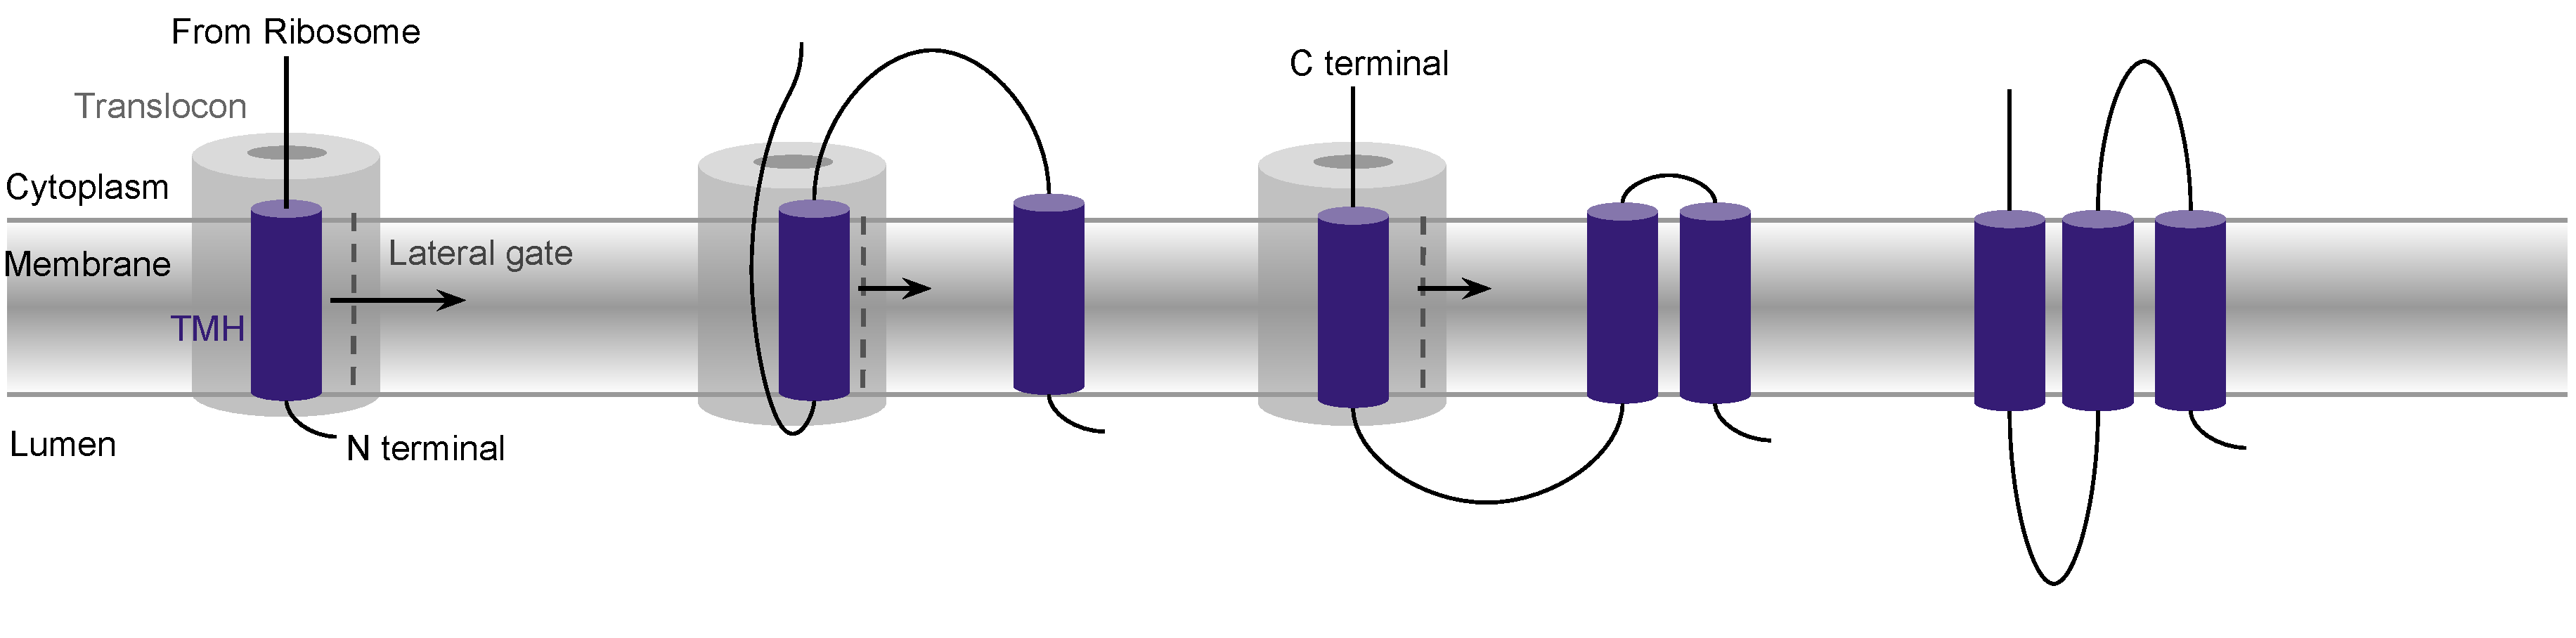
\includegraphics[width=1\textwidth]{multipass-folding/sequential-insertion}
        \captionof{figure}[A cartoon showing the generally accepted schematic of sequential multipass TMH insertion into the membranes.]{\textbf{A cartoon showing the generally accepted schematic of sequential multipass TMH insertion into the membranes.}
        The two key concepts are that, one at a time, the TMHs emerge from the ribosome into the translocon.
        This appearence of hydrophobicity triggers the lateral gate to open.
        As the nascent TMH is exposed to the membrane, it begins to partition.
        The downstream protein from the TMH is then threaded through the translocon until the next TMH is recognised.
        This implies that the TMHs ultimately have no meaningful interactions with one another until the protein has been threaded into the membrane and the multiple TMHs form a bundle.
}
\label{fig:sequential-insertion}
\end{figure}

\subsection{Ribsomes in the biogenesis of membrane proteins.}
Ribosomes translate mRNA sequences to amino acid chains and are present in all living cells, and indeed the ribosomal complexes presence and activity is for many used to define whether something is alive.
They are a highly conserved RNA-protein complex with a multitude of accessory proteins and targetting factors.

During translation of a \gls{tmp} protein, the \gls{srp} binds to the ribosome after recognising the nascent protein as a \gls{tmp}.
This complex then binds to the \gls{sr} in association with the membrane bound translocon.
The nascent peptide is then fed into the translocon as it is being translated; hence ``co-translational insertion''.

\begin{figure}[!ht]
\centering
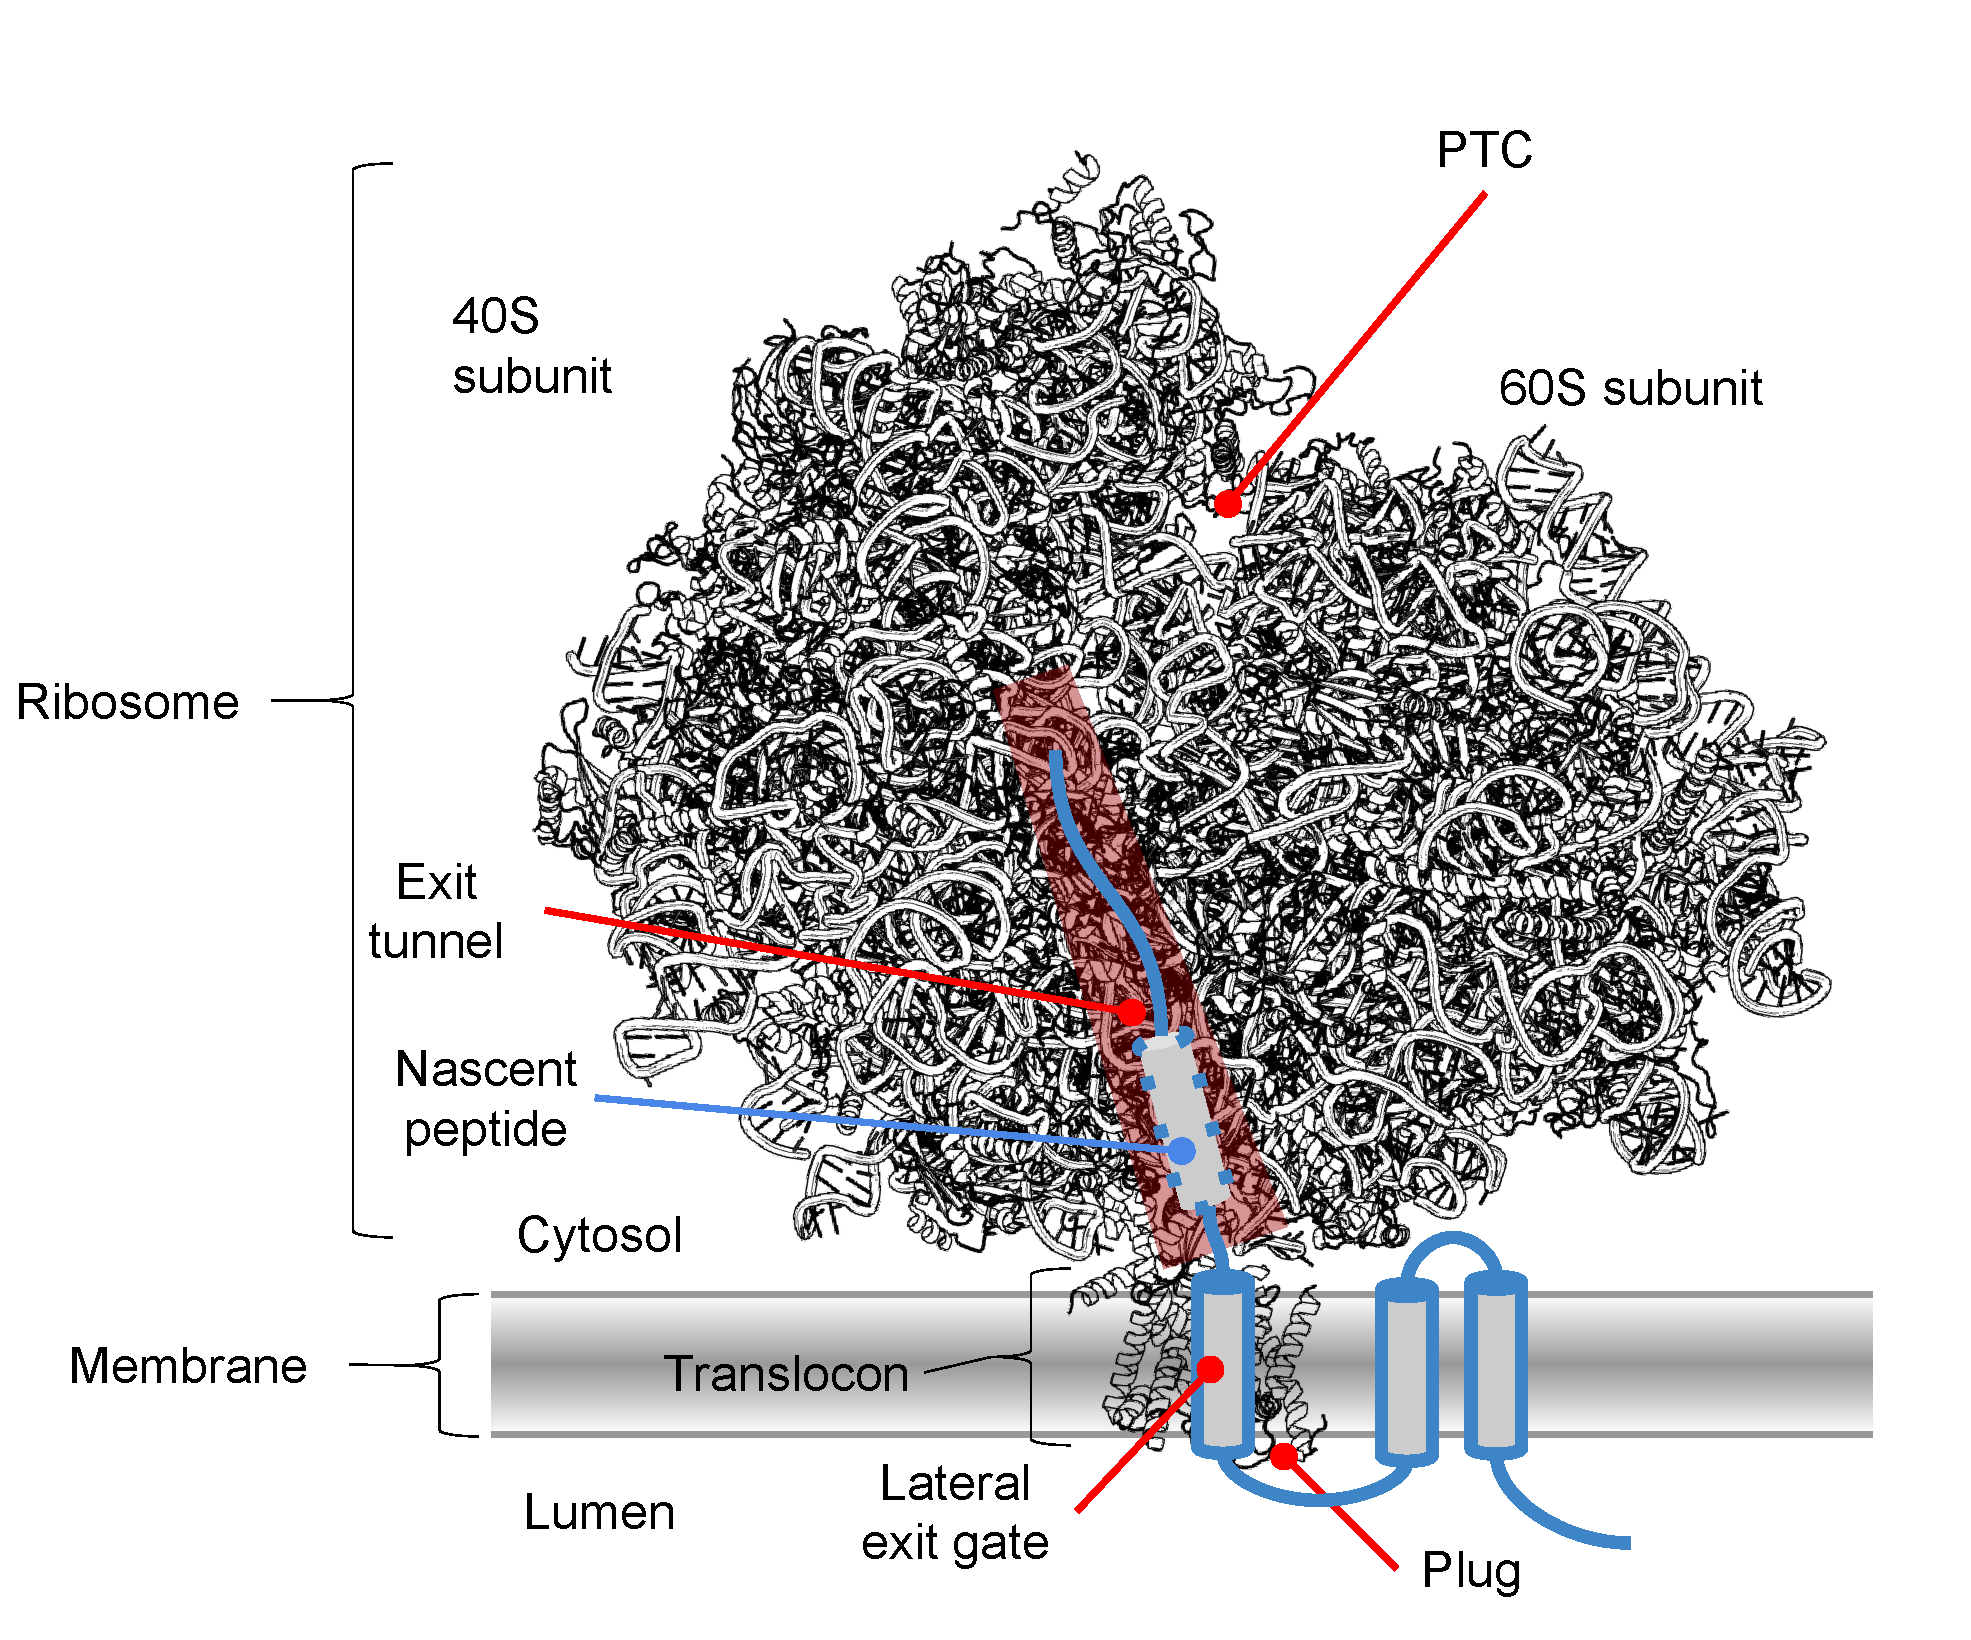
\includegraphics[width=1\textwidth]{multipass-folding/Ribosome-translocon-complex}
        \captionof{figure}[A cartoon of the ribosome in association with the translocon during insertion.]{\textbf{A cartoon of the ribosome in association with the translocon during insertion.}
}
\label{fig:Ribosome-translocon-complex}
\end{figure}

\gls{ap}s are typically 10-15 residues long that bind to the upper end of the ribosomal exit tunnel.
Once a specific mRNA codon is recognised, ribosomal stalling is induced \cite{Ito2010} and translation is halted unless a strong enough pulling force from the downstream insertion is acting on the nascent chain at that time \cite{Butkus2013}.
Several ``strengths'' of \gls{ap} have been identified.
For example, SecM from \textit{E. coli} is 17 residues long and relatively weak, whereas a mutated SecM from \textit{Mannheimia succiniciproducens}(Ms-Sup1) is much stronger and 8 residues long ending in a proline which will halt translation \cite{Ismail2012}.
There are several other SecM proteins of other strengths from various bacterial species \cite{Yap2009}.
Therefore \gls{ap}s are a technique that can be used to measure precise forces acting on a specific part of the nascent chain during co-transltaional membrane protein integration allowing the study of \gls{tmp} kinetics during insertion and folding.
Indeed the force profile of a single residue can now be obtained \textit{in vivo} \cite{Ismail2012}.
In an idealised \gls{tmh} segment composed of alanine and leucine being inserted into \textit{E. coli} membrane through SecM \gls{ap} with SDS-PAGE, hydrophobicity is more able to overcome the arrest peptide when it is near the N-terminal (of an N-terminal-inside \gls{tmh}) \cite{Ismail2012}.
This could be either the \gls{tmh} finally coming into contact with the cytoplasmic face of the lipid bilayer, or an interaction between the N-terminal and the tip of the lateral gate as previosuly shown in Sec61; part of a pre-integration \gls{tmh} interrogation \cite{MacKinnon2014}.

The journey of the \gls{tmh} through this machinery has been studied using both crosslinking experiments and the relatively new technique of \gls{ap}s \cite{Cymer2015}.

Accessibility assays and an improved intramolecular crosslinking assay showed that the helical transmembrane S3b–S4 hairpin (the “paddle”) of a voltage-gated potassium (Kv) forms in the ribosome tunnel \cite{Tu2014}.
Ribosomal folding of the \gls{tmh}s in Kv1.3, a potassium channel, is maintained in the translocon \cite{Tu2010}.
Therefore, some of the final structural folded elements of the voltage sensor domain occurs within the ribosomal exit tunnel.

Furthermore, it has recently been suggested that larger structures fold as the ribosomal exit tunnel widens \cite{Kudva2018}.
This size dependent folding was observed by using the SecM translational \gls{ap}.
Two ribosome mutants were compared (uL23 that is close to the exit tunnel and uL24 deletions which is a hairpin loop that obstructs the tunnel exit.) zinc finger folds deeper in uL23 mutant than wildtype (but not uL24) and a 100 residue domain folds deeper than the uL24 mutant (but not the uL23) \cite{Kudva2018}.

The ribosomal tunnel also speeds up elongation of neutral and negatively-charged peptides.
This is attributed to the sporadic negative patches within the ribosomal exit tunnel \cite{Lu2008}.

The ribosome clearly has the potential to prefold motifs and small domains before translocon insertion.

\subsection{Co-operative insertion}
Multiple \gls{tmh}s in a nascent protein can be associated with the eukaryotic translocon simultaneously.
It was shown that \gls{tmh}s can stay inassociation with the translocon in order to mediate integration of downstream \gls{tmh}s demonstrated by crosslinking analysis \cite{Sadlish2005, Cross2009}.
Not only this, but it was shown that there is a direct interaction between the \gls{tmh}s; more recently \gls{ap}s were used to show pulling forces between a \gls{tmh} and more C-terminally located \gls{tmh} during the C-terminal \gls{tmh} membrane partitioning from the translocon \textit{in vivo} \cite{Cymer2013}.
This could be facilitated during the probing of a \gls{tmh} from the translocon as the lateral gate ``cracks'' open in an intermediate stage before the \gls{tmh} satisfies the full hydrophobic requirements to open the gate fully, an intermediate stage observed in a SecY crystal structure \cite{Egea2010}.

\section{Results and discussion}

\subsection{Large contrasts in TMH hydrophobicity occurs in channels and receptors.}
In order to identify which type of \gls{tmp} there may be potentially large numbers of cooperateive \gls{tmh}, the hydrophobicities for all \gls{tmh}s in a redudant version of SwissProt were calculated according to the Kyte \& Dolittle hydropathy scale \cite{Kyte1982}.
The absolute difference between each sequentially adjacent \gls{tmh} was calculated.
The full list, along with the 0.1\% \gls{tmh} pair were submitted to PANTHER \cite{Mi2017}.

\begin{figure}[!ht]
\centering
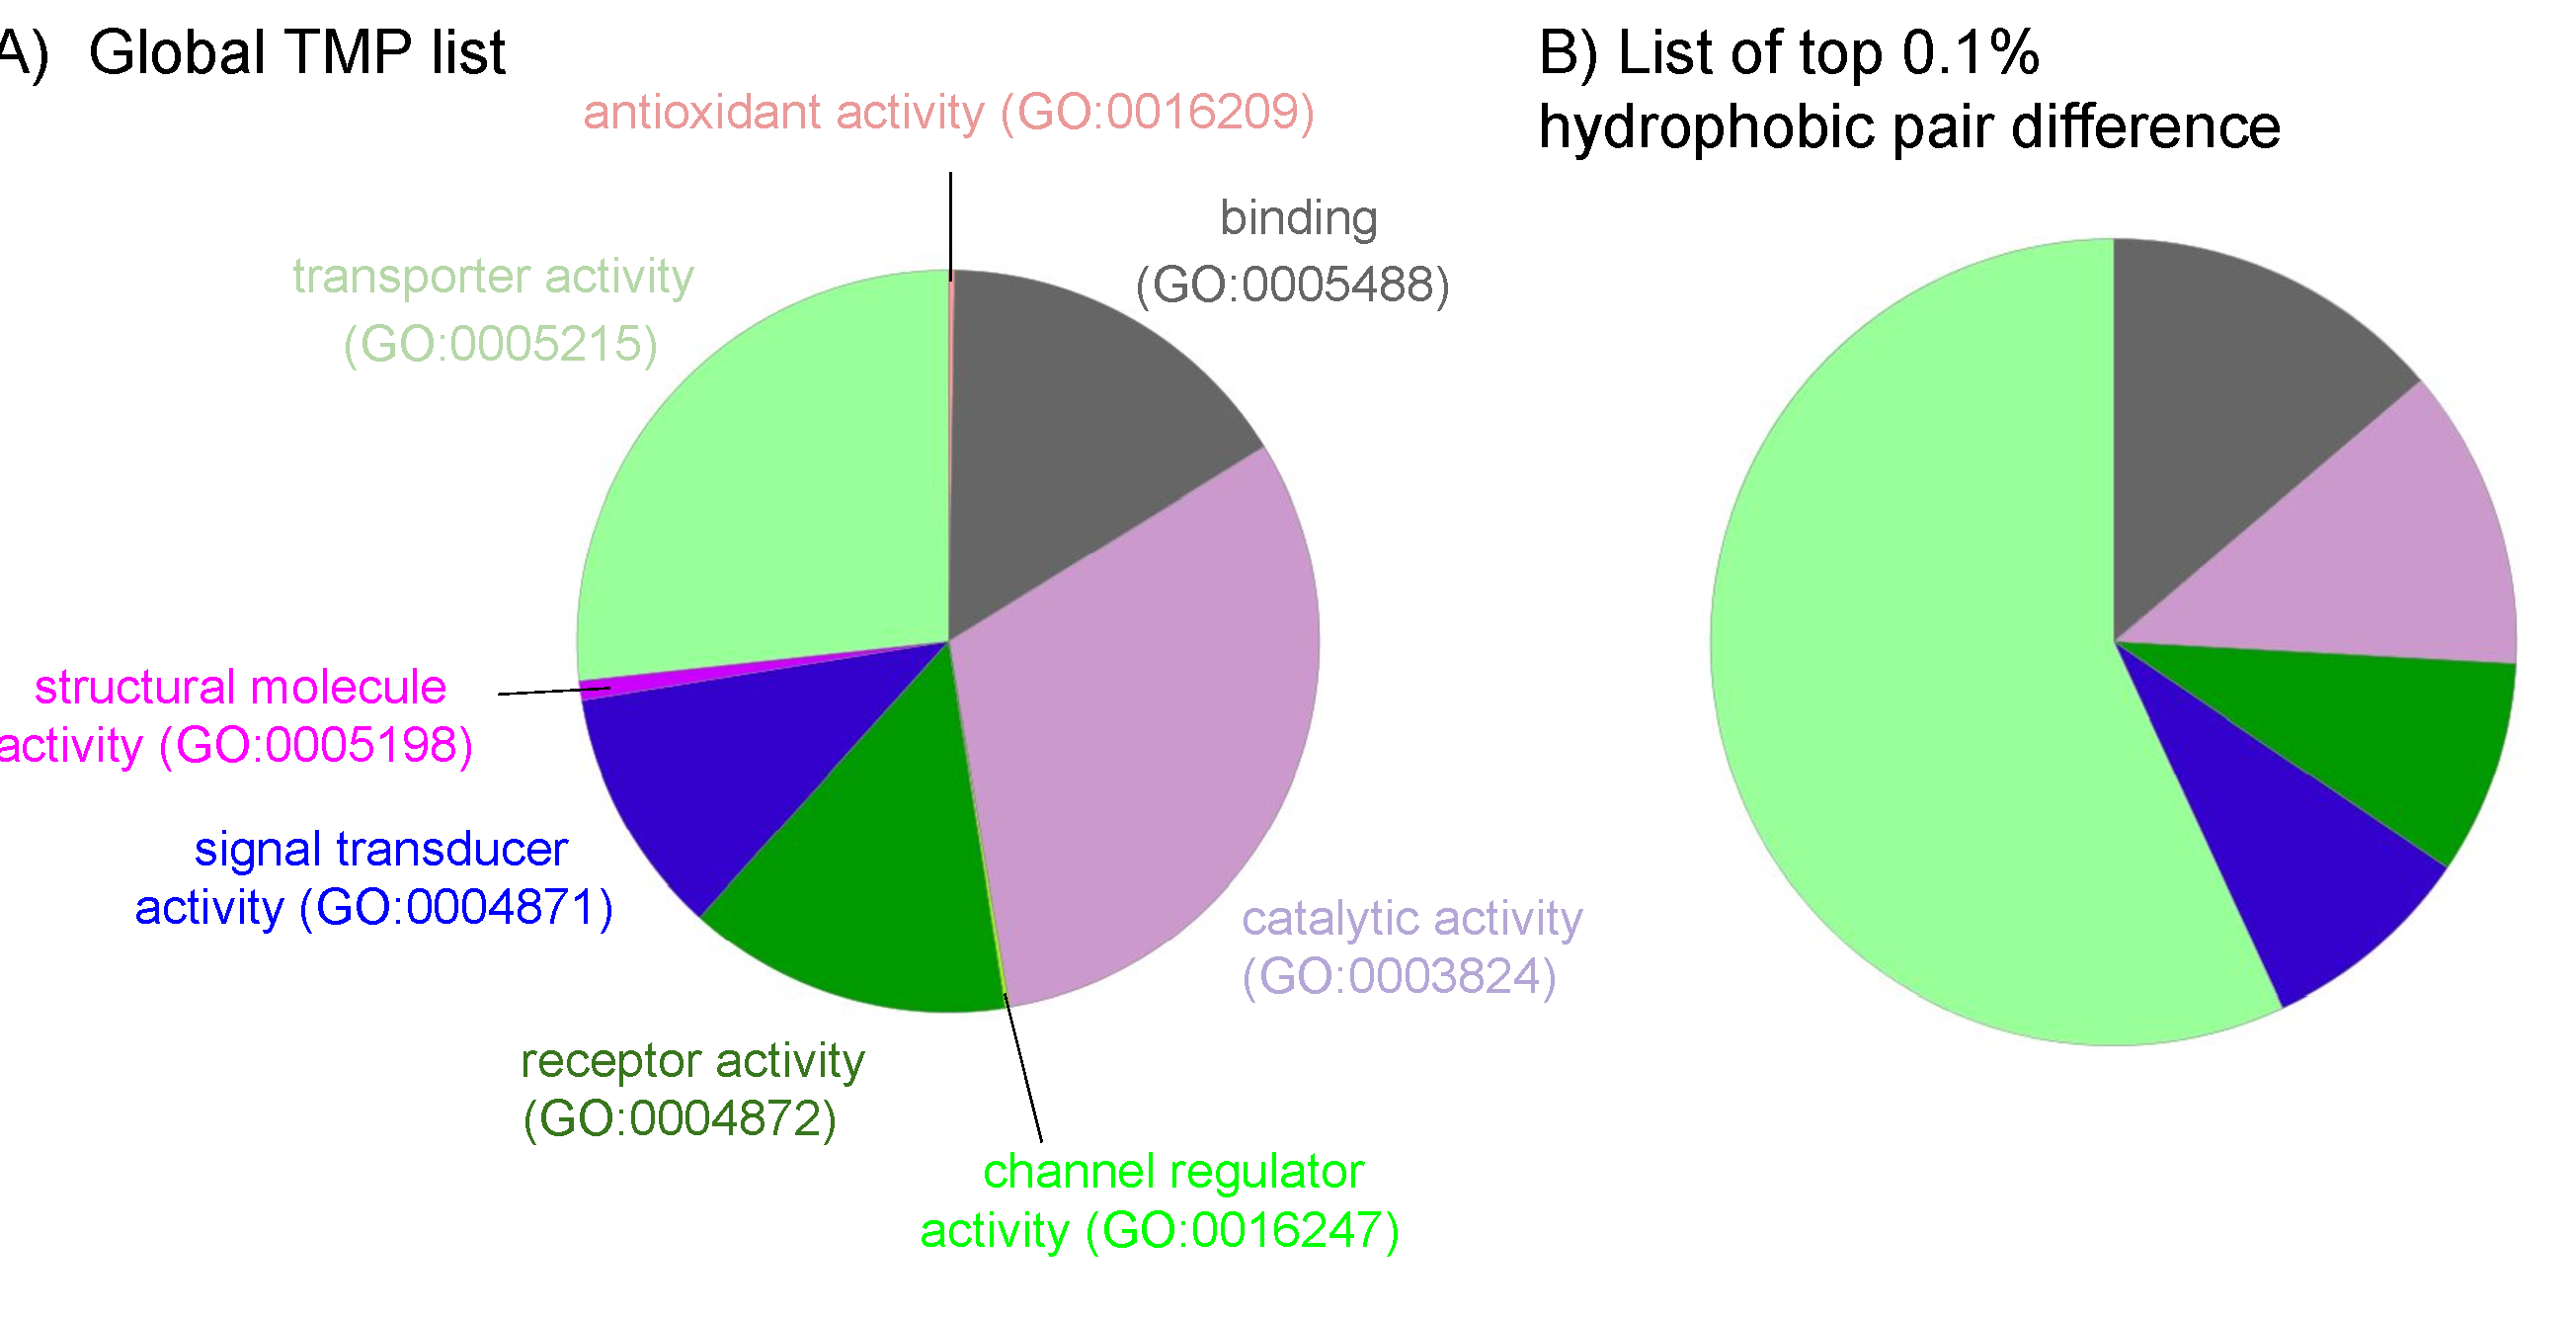
\includegraphics[width=1\textwidth]{multipass-folding/good-bad-ontology}
		\captionof{figure}[Pie charts of a non-redundant list of TMPs compared to a list of TMPs containing the most hydrophobically different TMH pais.]{\textbf{Pie charts of a non-redundant list of TMPs compared to a list of TMPs containing the most hydrophobically different TMH pairs.}}

\label{fig:good-bad-ontology}
\end{figure}

%Need percentage decreases

\subsection{GPCRs contain high a conserved relatively polar TMH}

\begin{figure}[!ht]
\centering
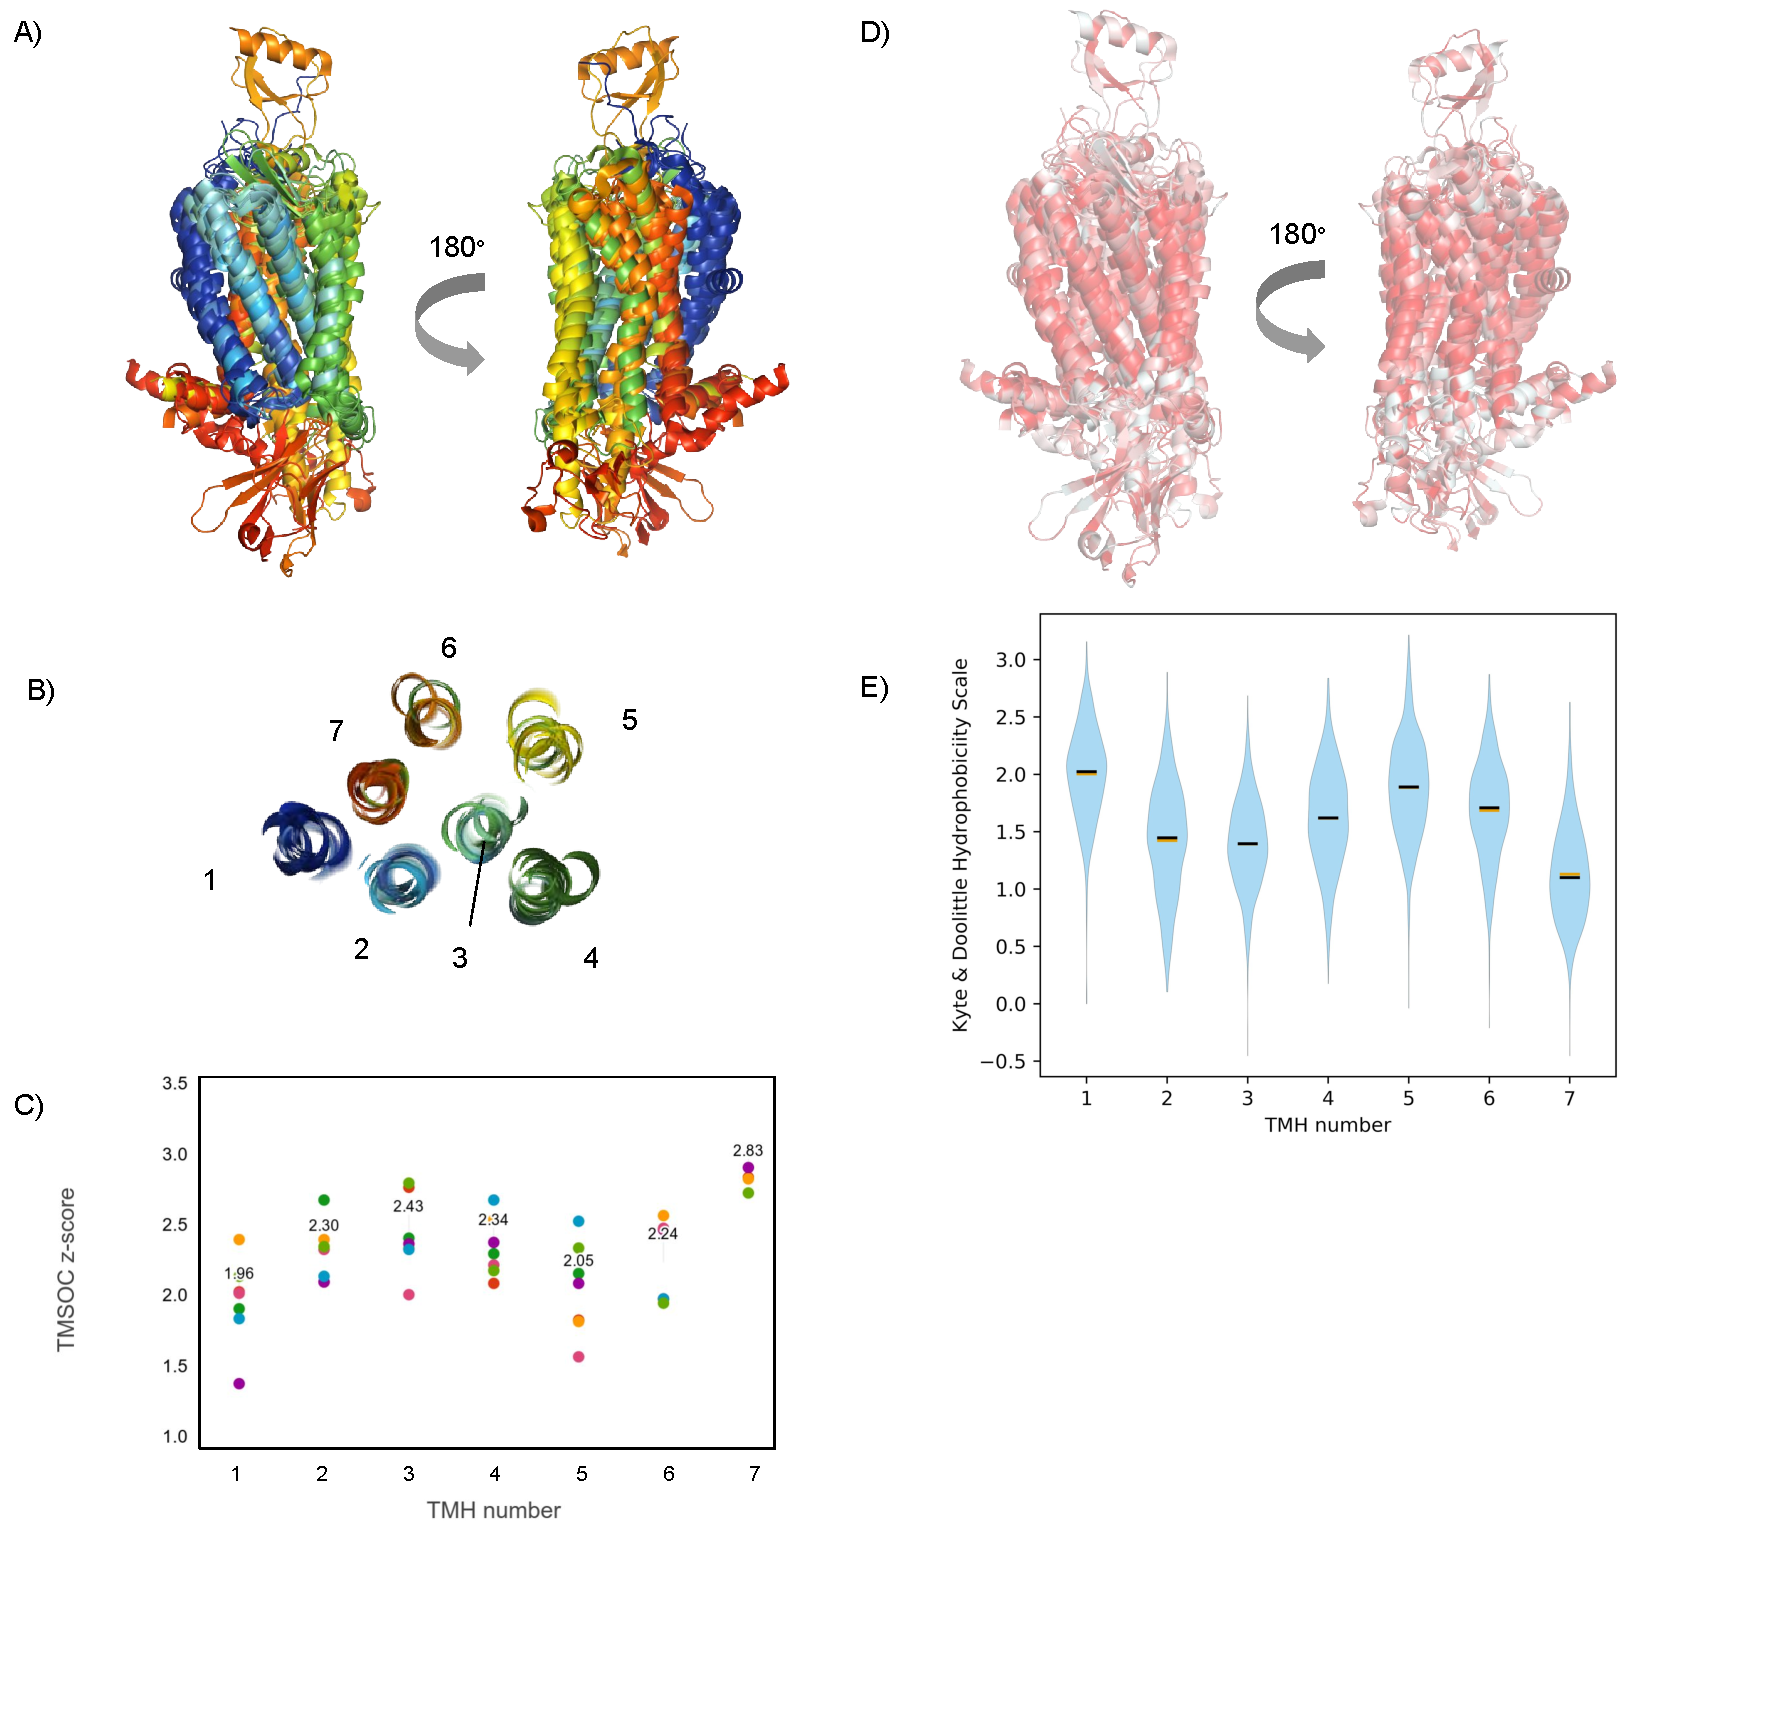
\includegraphics[width=1\textwidth]{multipass-folding/GPCR-structures}
		\captionof{figure}[The hydrophobicity and complexity of GPCR TMHs.]{\textbf{The hydrophobicity and complexity of GPCR TMHs.}}

\label{fig:GPCR-structures}
\end{figure}

GPCR distribution tables for complexity and hydrophobicity
Graphs of complexity and hydrophobicity distributions
Show there are step changes in GPCRs from Bahadur
Supplementary tables for additional stats tests and hydrophobicities

\gls{gpcr}s are a diverse family of membrane surface receptors with 7 \gls{tmh} segments.
GPCRs have long be known to be overrepresented among genomes \cite{Remm2000}.
They have adapted to respond to a wide range of specific signals ranging from macromolecules to photons.
The specific signal triggers a conformational change of the \gls{gpcr} that is translated across the membrane.
\gls{gpcr}s have been associated with tumerigenesis \cite{OHayre2013}, metastasis \cite{Singh2015} and in cancers \cite{Bar-Shavit2016} and are a potential target for therapies \cite{Arakaki2018}.
Their ubiquitous presence in cellular life and medical relevance makes them an important topic of study.

Opsins are a group of light sensitive \gls{gpcr}s.
It was shown by cross linking studies that opsin \gls{tmh}s 5-7 are retained in the \gls{er} translocon and only parition once biosynthesis is complete \cite{Ismail2008}.
The timing of this partitioning is controlled by the hydrophobicity of the \gls{tmh}, not protein length or the relative position of the \gls{tmh} within the protein.
Although artificially extending the C-terminal did not result release of the \gls{tmh}s, by replacing native \gls{tmh} 7 with a more hydrophobic \gls{tmh}, the speed of insertion was decreased.
\gls{tmh}s 1-4 are inserted independently, and the 5-7 \gls{tmh}s partition into the membrane at the same time.

\subsection{The pattern is present for GPCR subfamilies}
Figure of complexity distributions with Rhodopsin like, Secretin, metabotropic glutamate, Fungal mating, cyclic AMP, Frizzled and smooth.
Bahadur tables also

\begin{figure}[!ht]
\centering
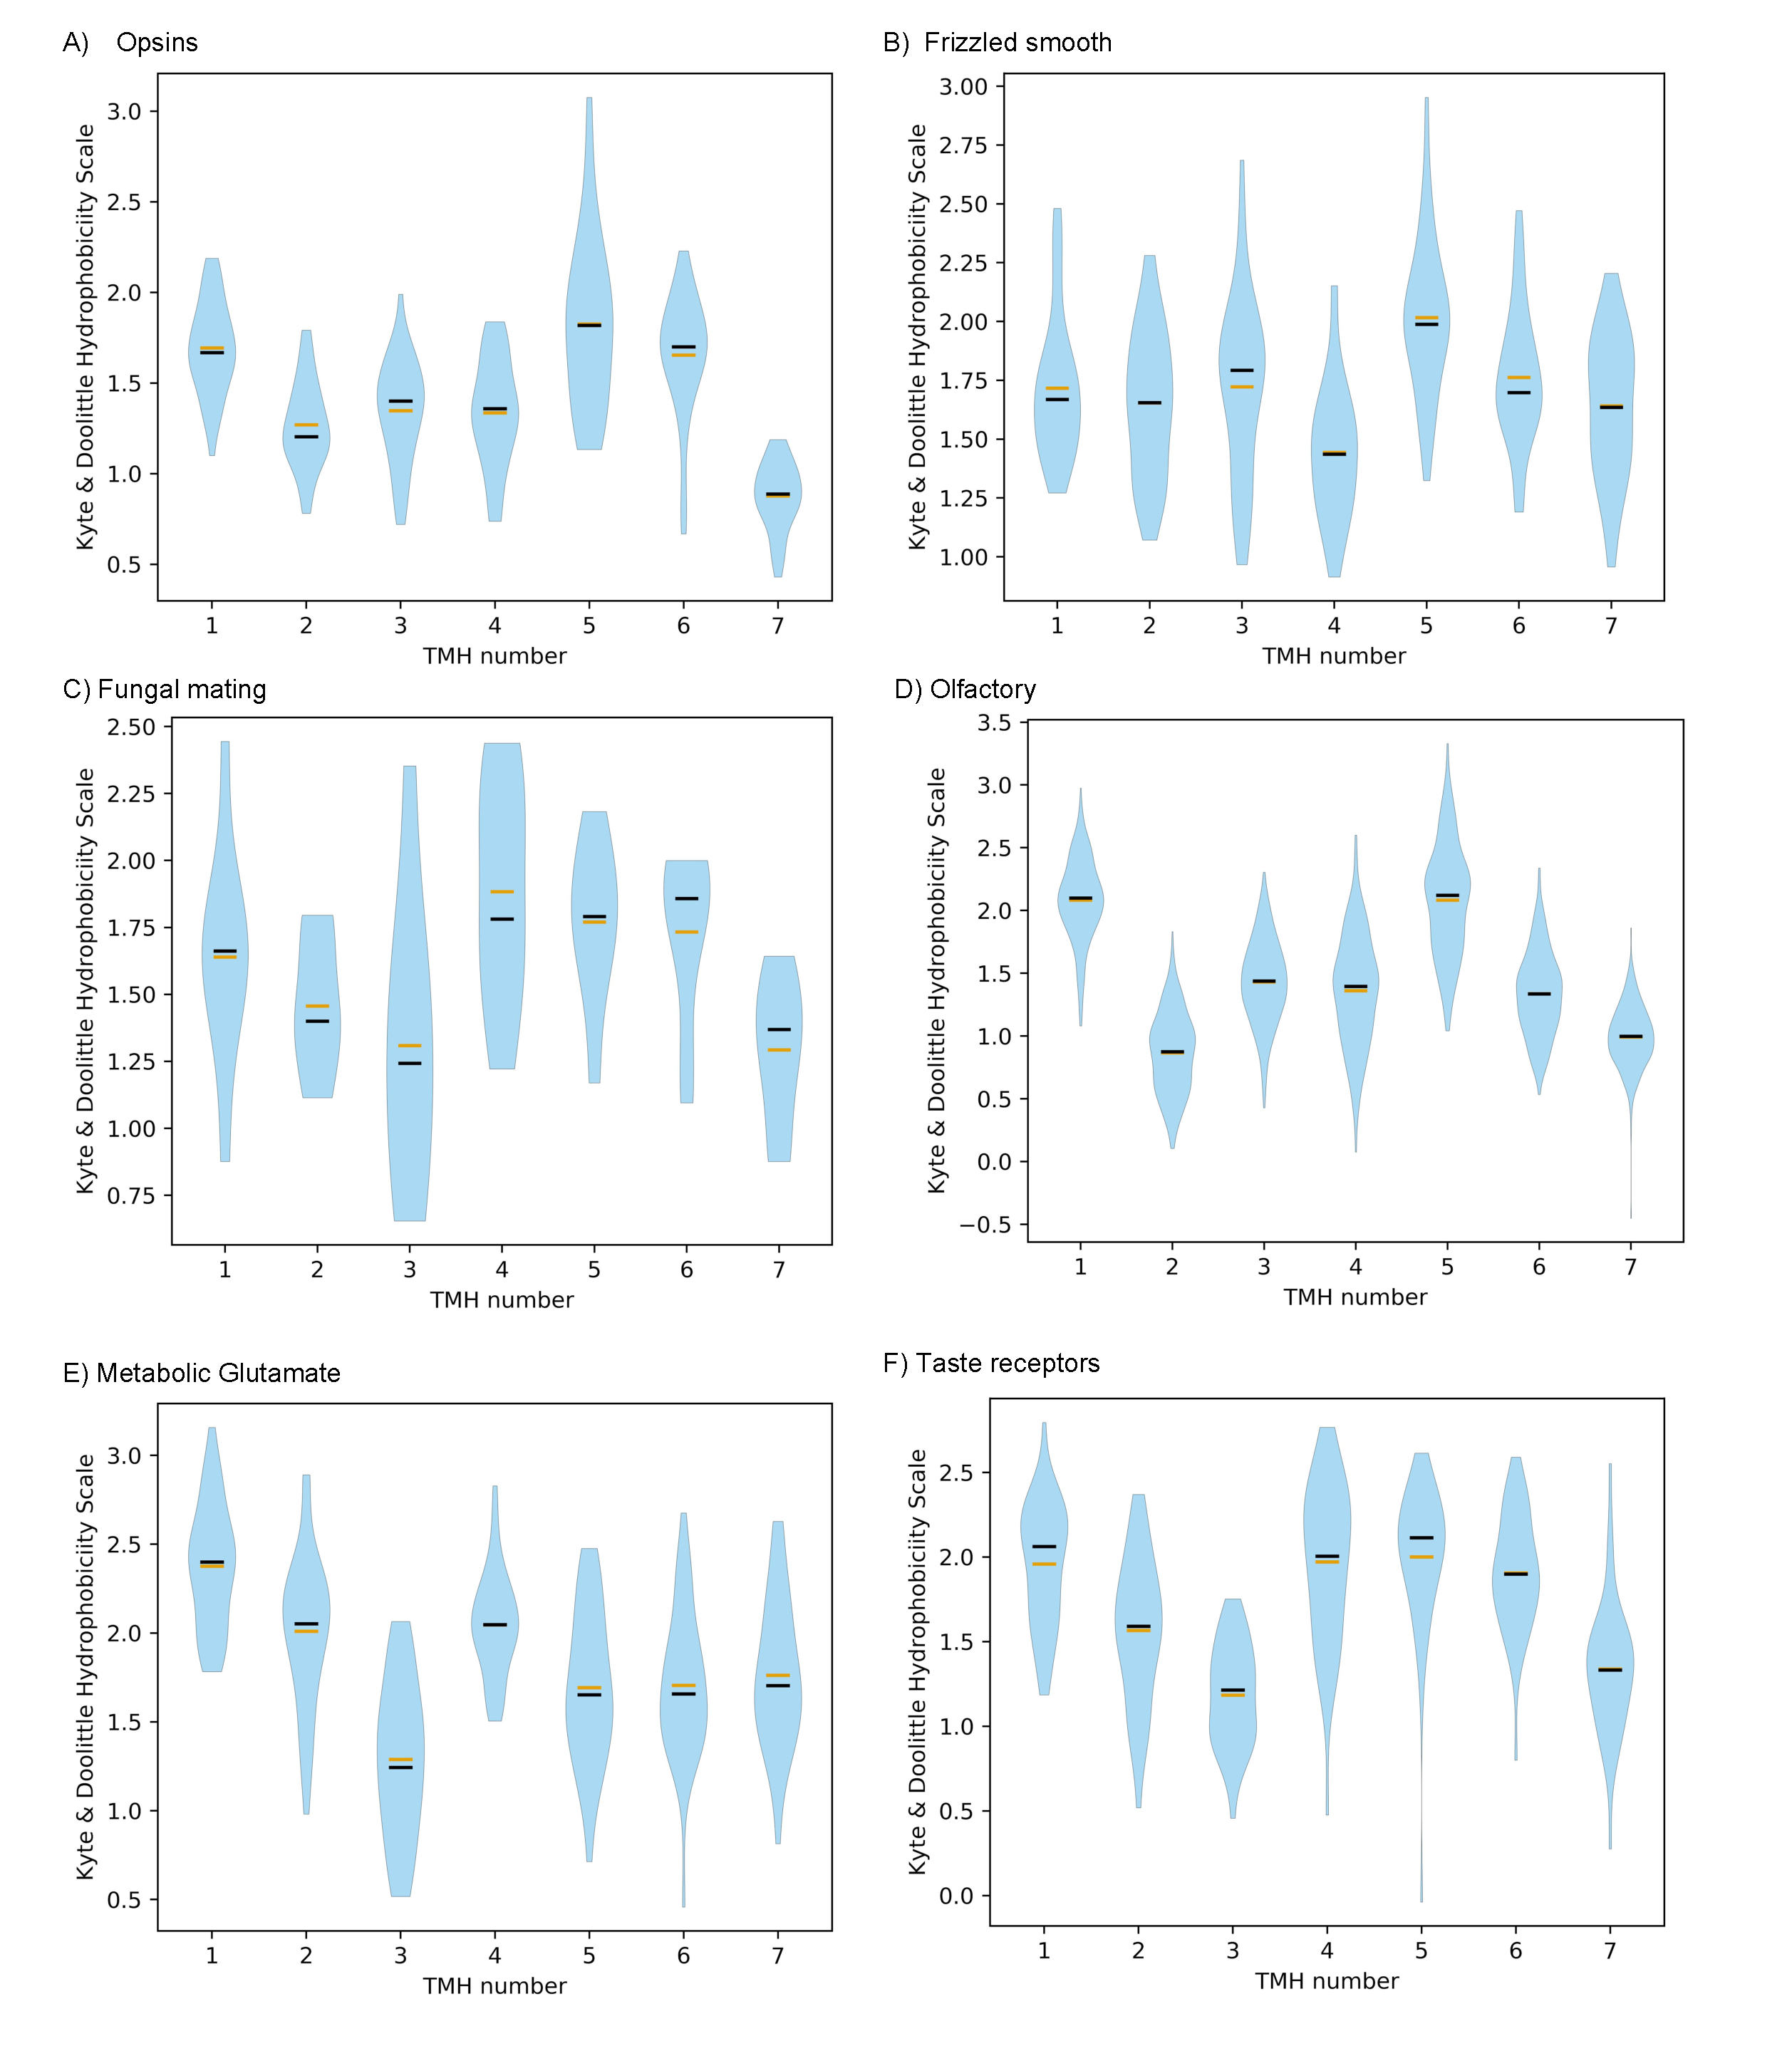
\includegraphics[width=1\textwidth]{multipass-folding/KD-GPCR}
		\captionof{figure}[The hydrophobicity of TMHs in GPCR subfamilies.]{\textbf{The hydrophobicity of TMHs in GPCR subfamilies.}}

\label{fig:KD-GPCR}
\end{figure}


\subsection{Ion channels contain polar-hydrophobic TMH pairs/groups}

\begin{figure}[!ht]
\centering
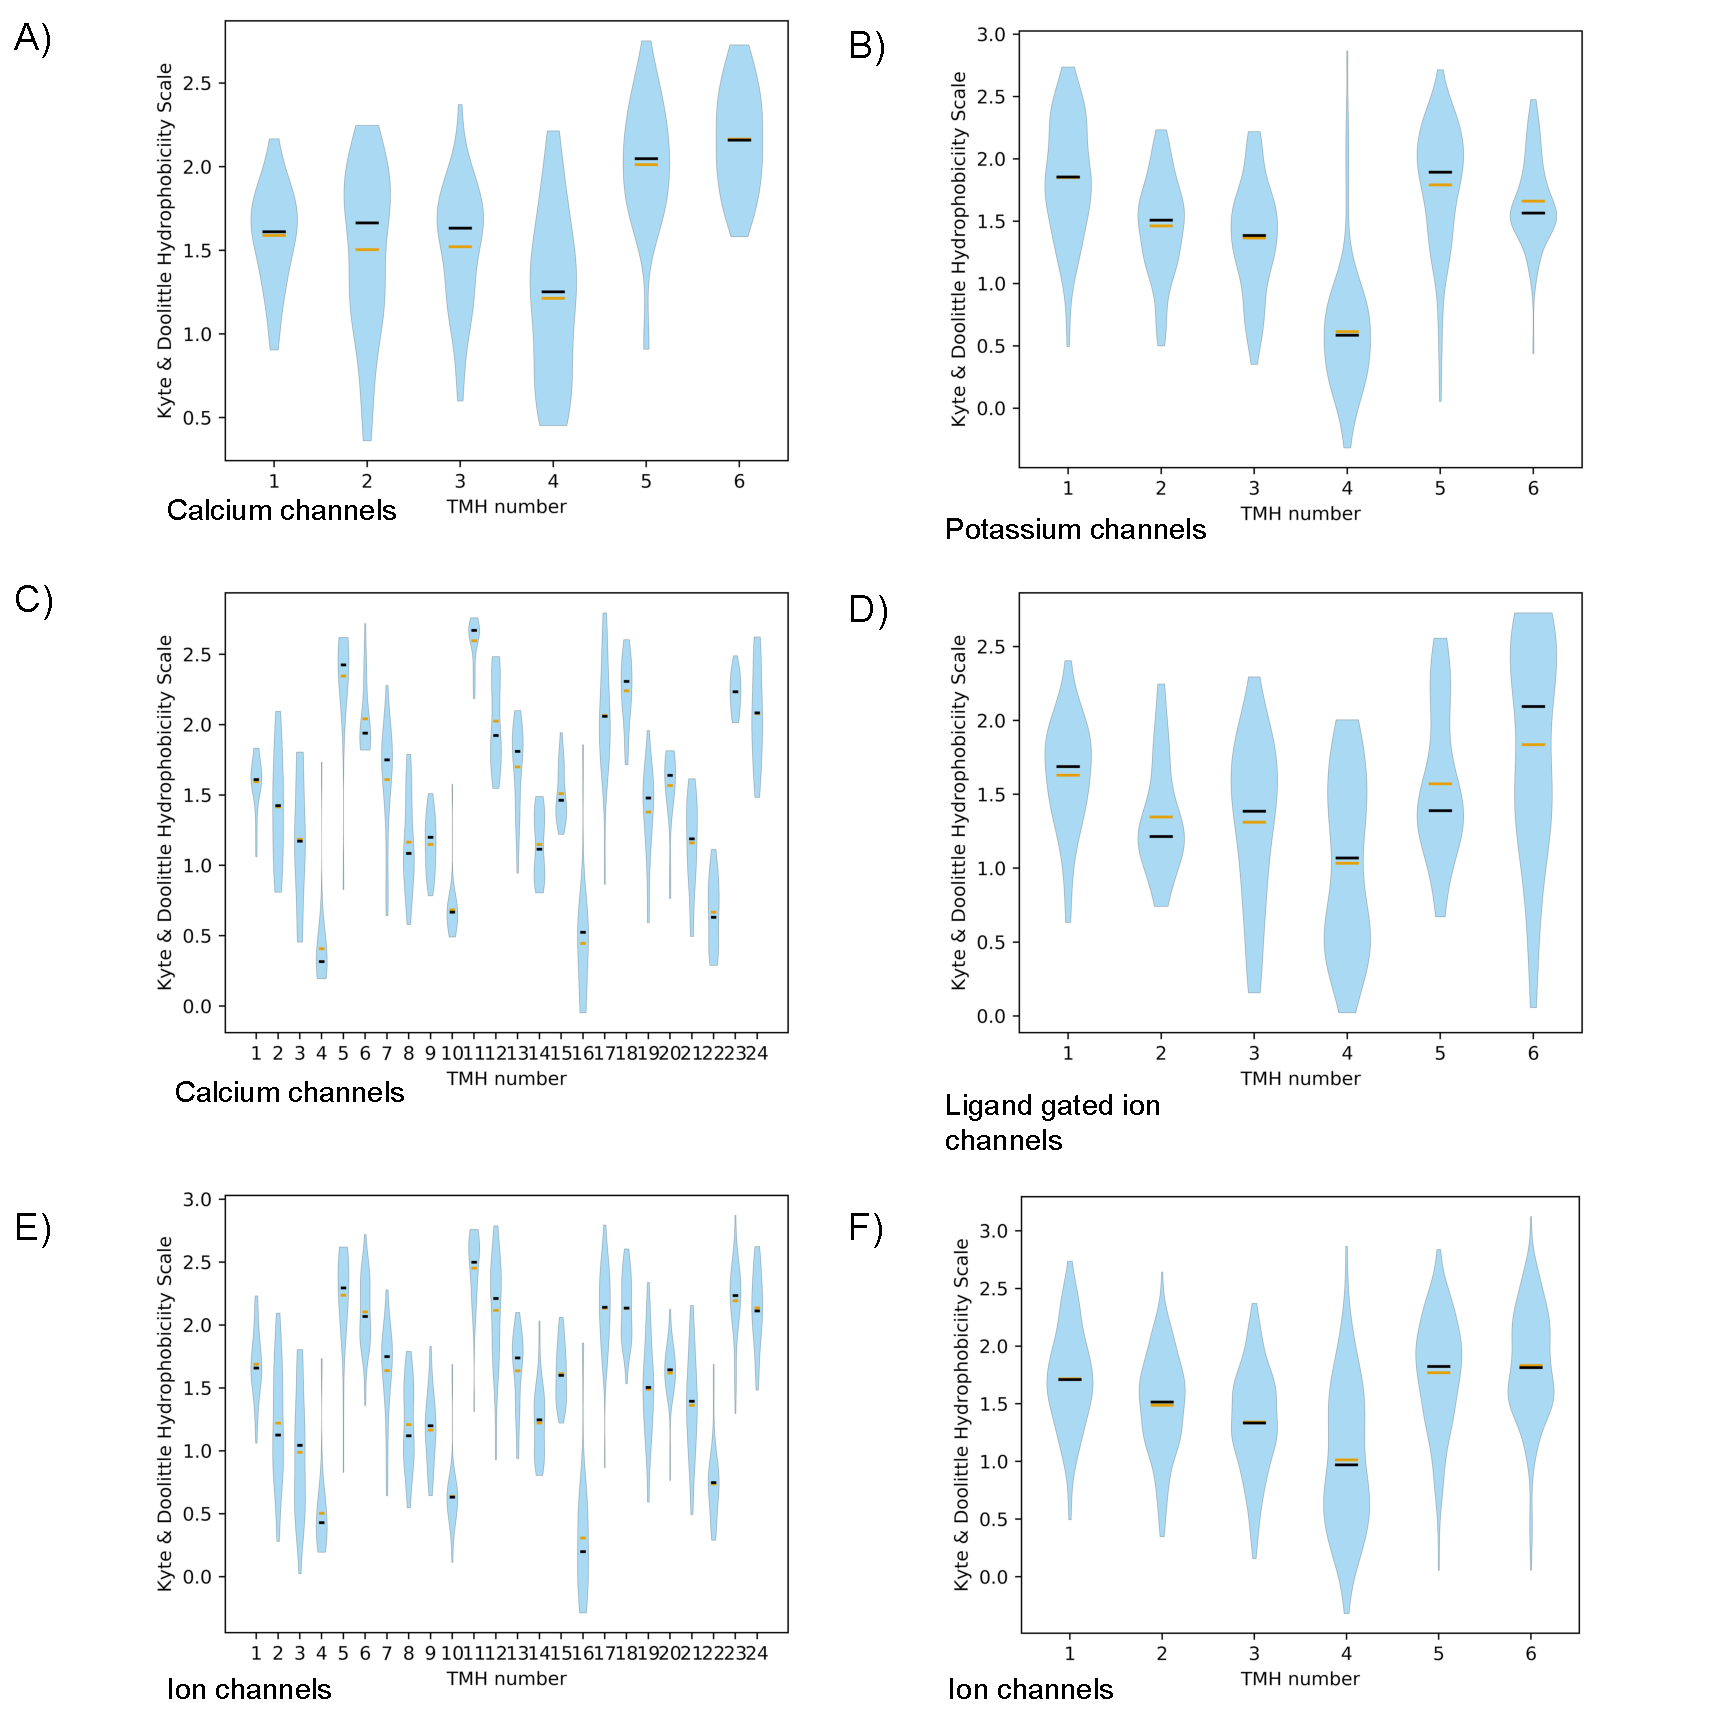
\includegraphics[width=1\textwidth]{multipass-folding/KD-ion-channels}
		\captionof{figure}[The hydrophobicity of TMHs in ion channels.]{\textbf{The hydrophobicity of TMHs in ion channels.}}

\label{fig:KD-ion-channels}
\end{figure}

Another example of cooperative \gls{tmh} insertion is that of the 3rd and 4th \gls{tmh} of the potassium channel (shaker family) which was shown to insert either sequentially or cotranslationally \cite{Zhang2007, Cymer2015}.
This is especially notable in the case of KAT1, that is a plant K$_v$ channel that is thought to mediate long-term potassium influx into guard cells causing the stomata to open.
In the case of KAT1, N-glycosylation of various mutant fusion KAT1 constructs revealed that there is no choice of sequential insertion since \gls{tmh} 3 and 4 have no insertion potential and no topogenic functions themselves \cite{Sato2002, Sato2003}.
In \gls{tmh} 4 this is due to the charged residues making it relatively polar.
However, previous experimentation in Kv1.3 had found that while \gls{tmh} 4 did not initiate insertion, it did have insertion potential, and that when constgructs contained multiple \gls{tmh}s, membrane insertion efficiency increased \cite{Tu2000}.
Without the ability to stop the translation through the translocon and form a \gls{tmh}, it was suggested that a different means was needed than classic sequential insertion, and even that \gls{tmh} 3 and 4 are integrated by the translocon at the same time post-translationally, i.e the \gls{tmh}s are folded prior to insertion \cite{Sato2003}.
They achieve this in part becase the previous \gls{tmh}s 1 and 2 form a firm ``base'' within the membrane environment.

\subsection{The prevelance of this amongst all TMPs.}


\begin{figure}[!ht]
\centering
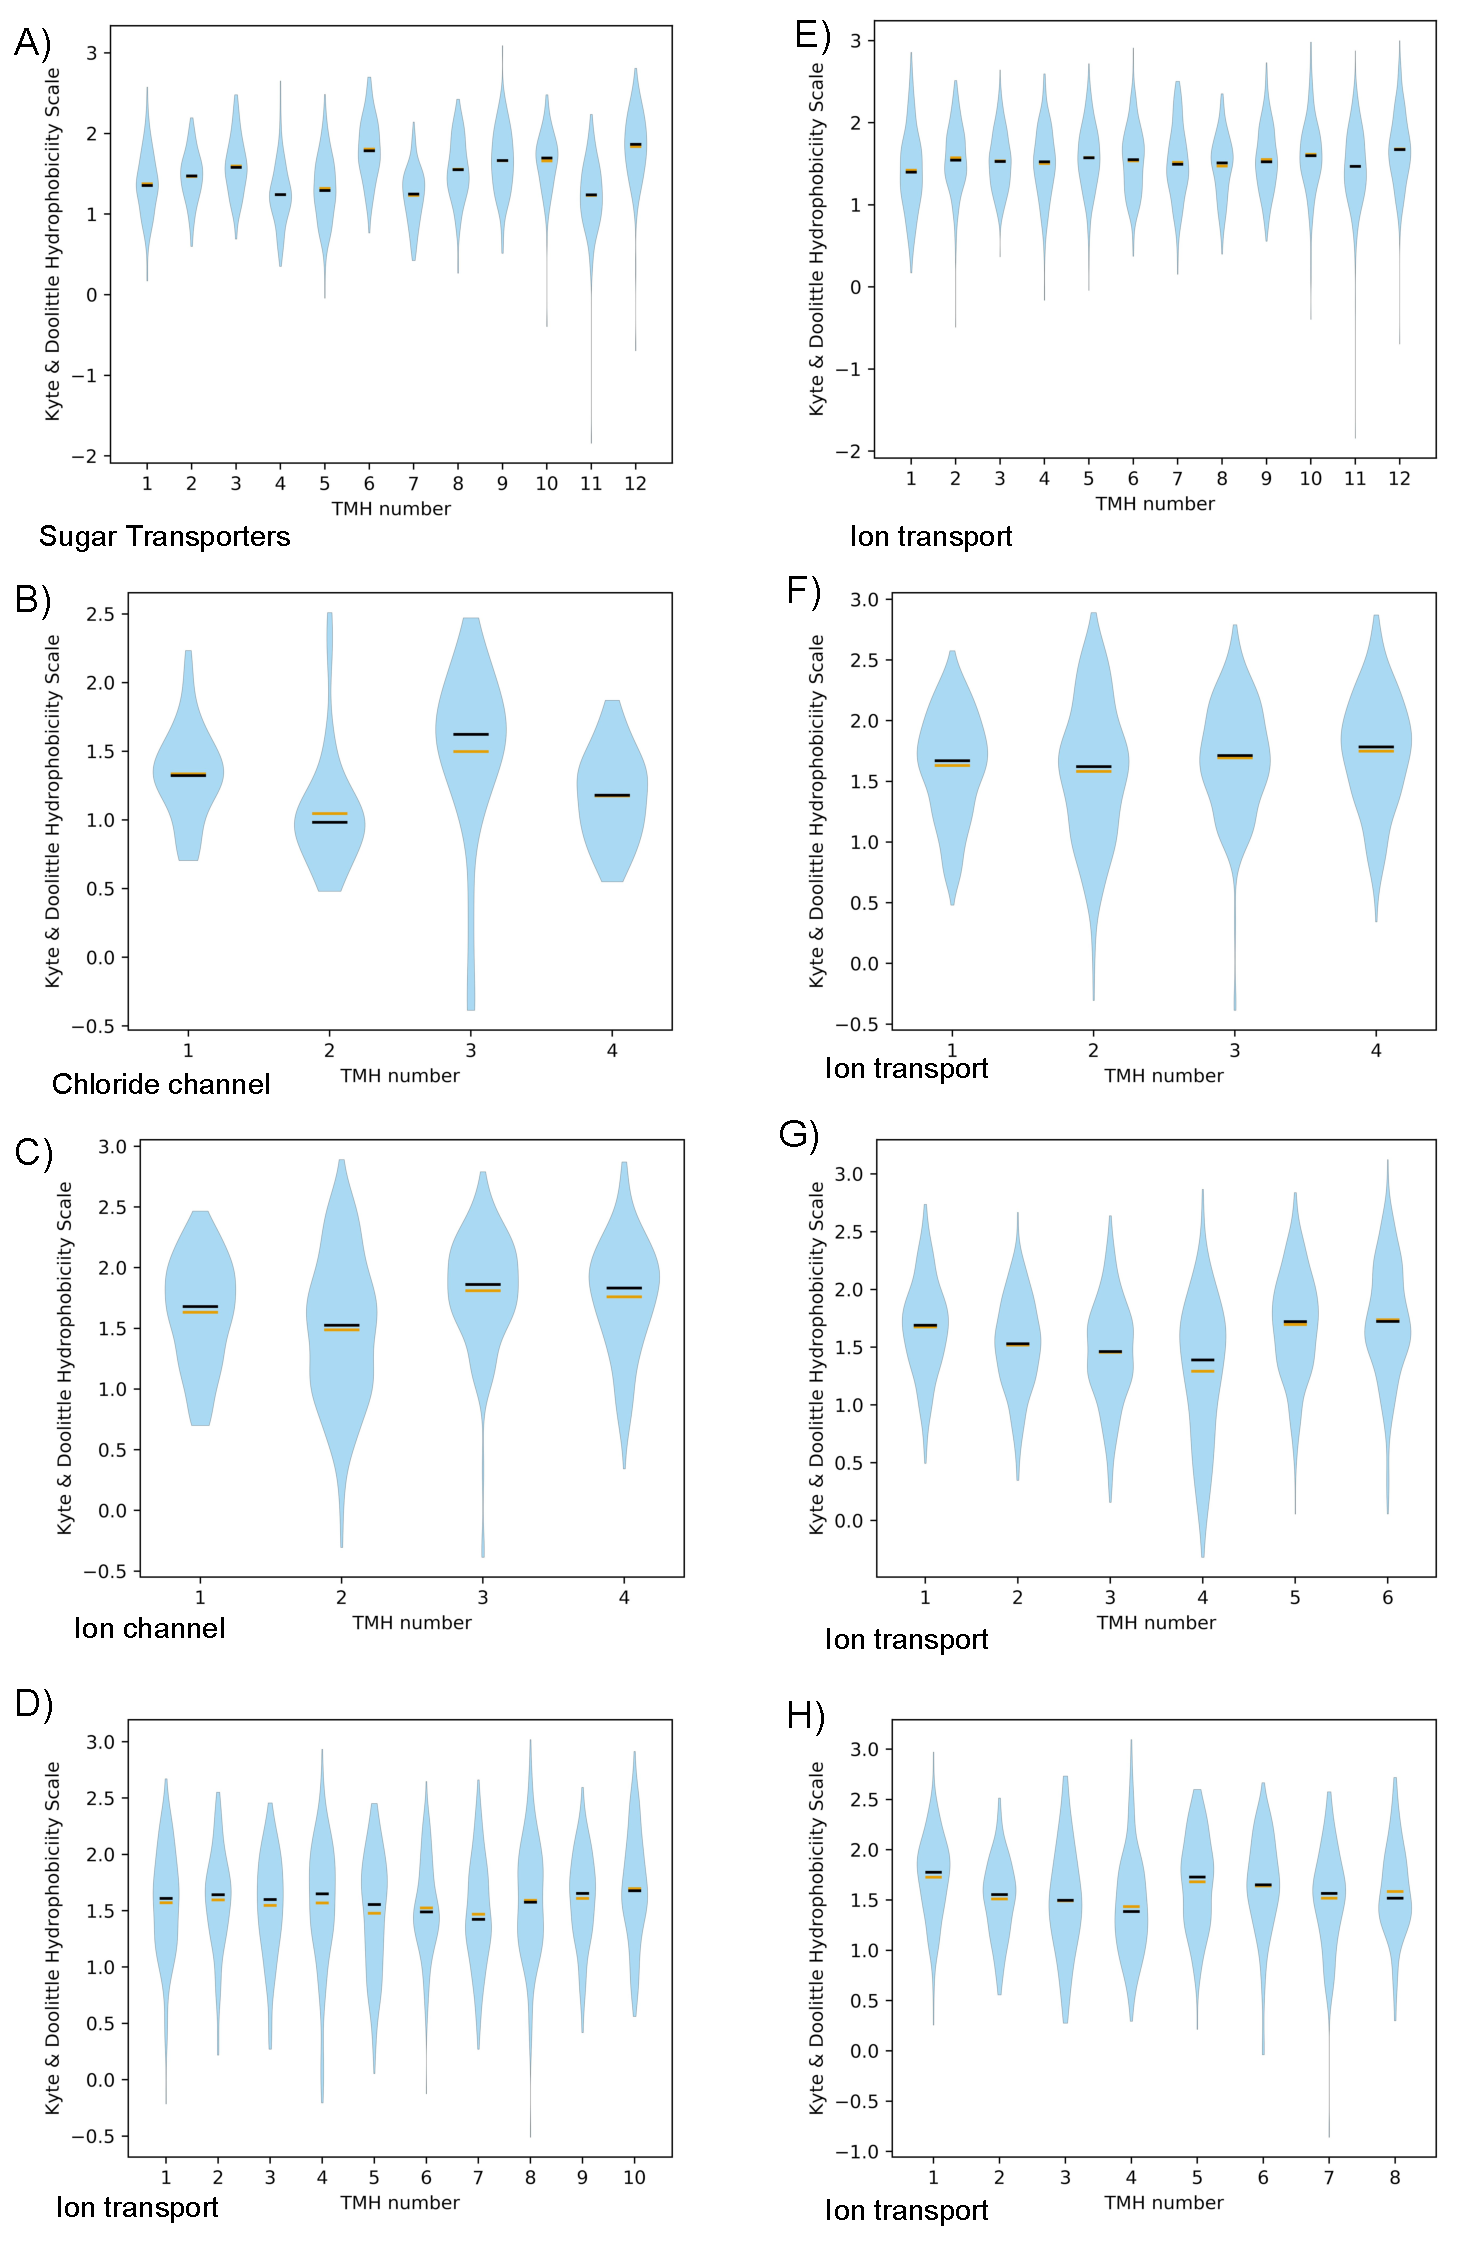
\includegraphics[width=0.8\textwidth]{multipass-folding/other-groups-good-bad}
		\captionof{figure}[Other large TMP groups with no apparrent polar-hydophobic groups.]{\textbf{Other large TMP groups with no apparrent polar-hydophobic groups.}}

\label{fig:other-groups-good-bad}
\end{figure}

\section{Summary}

\begin{figure}[!ht]
\centering
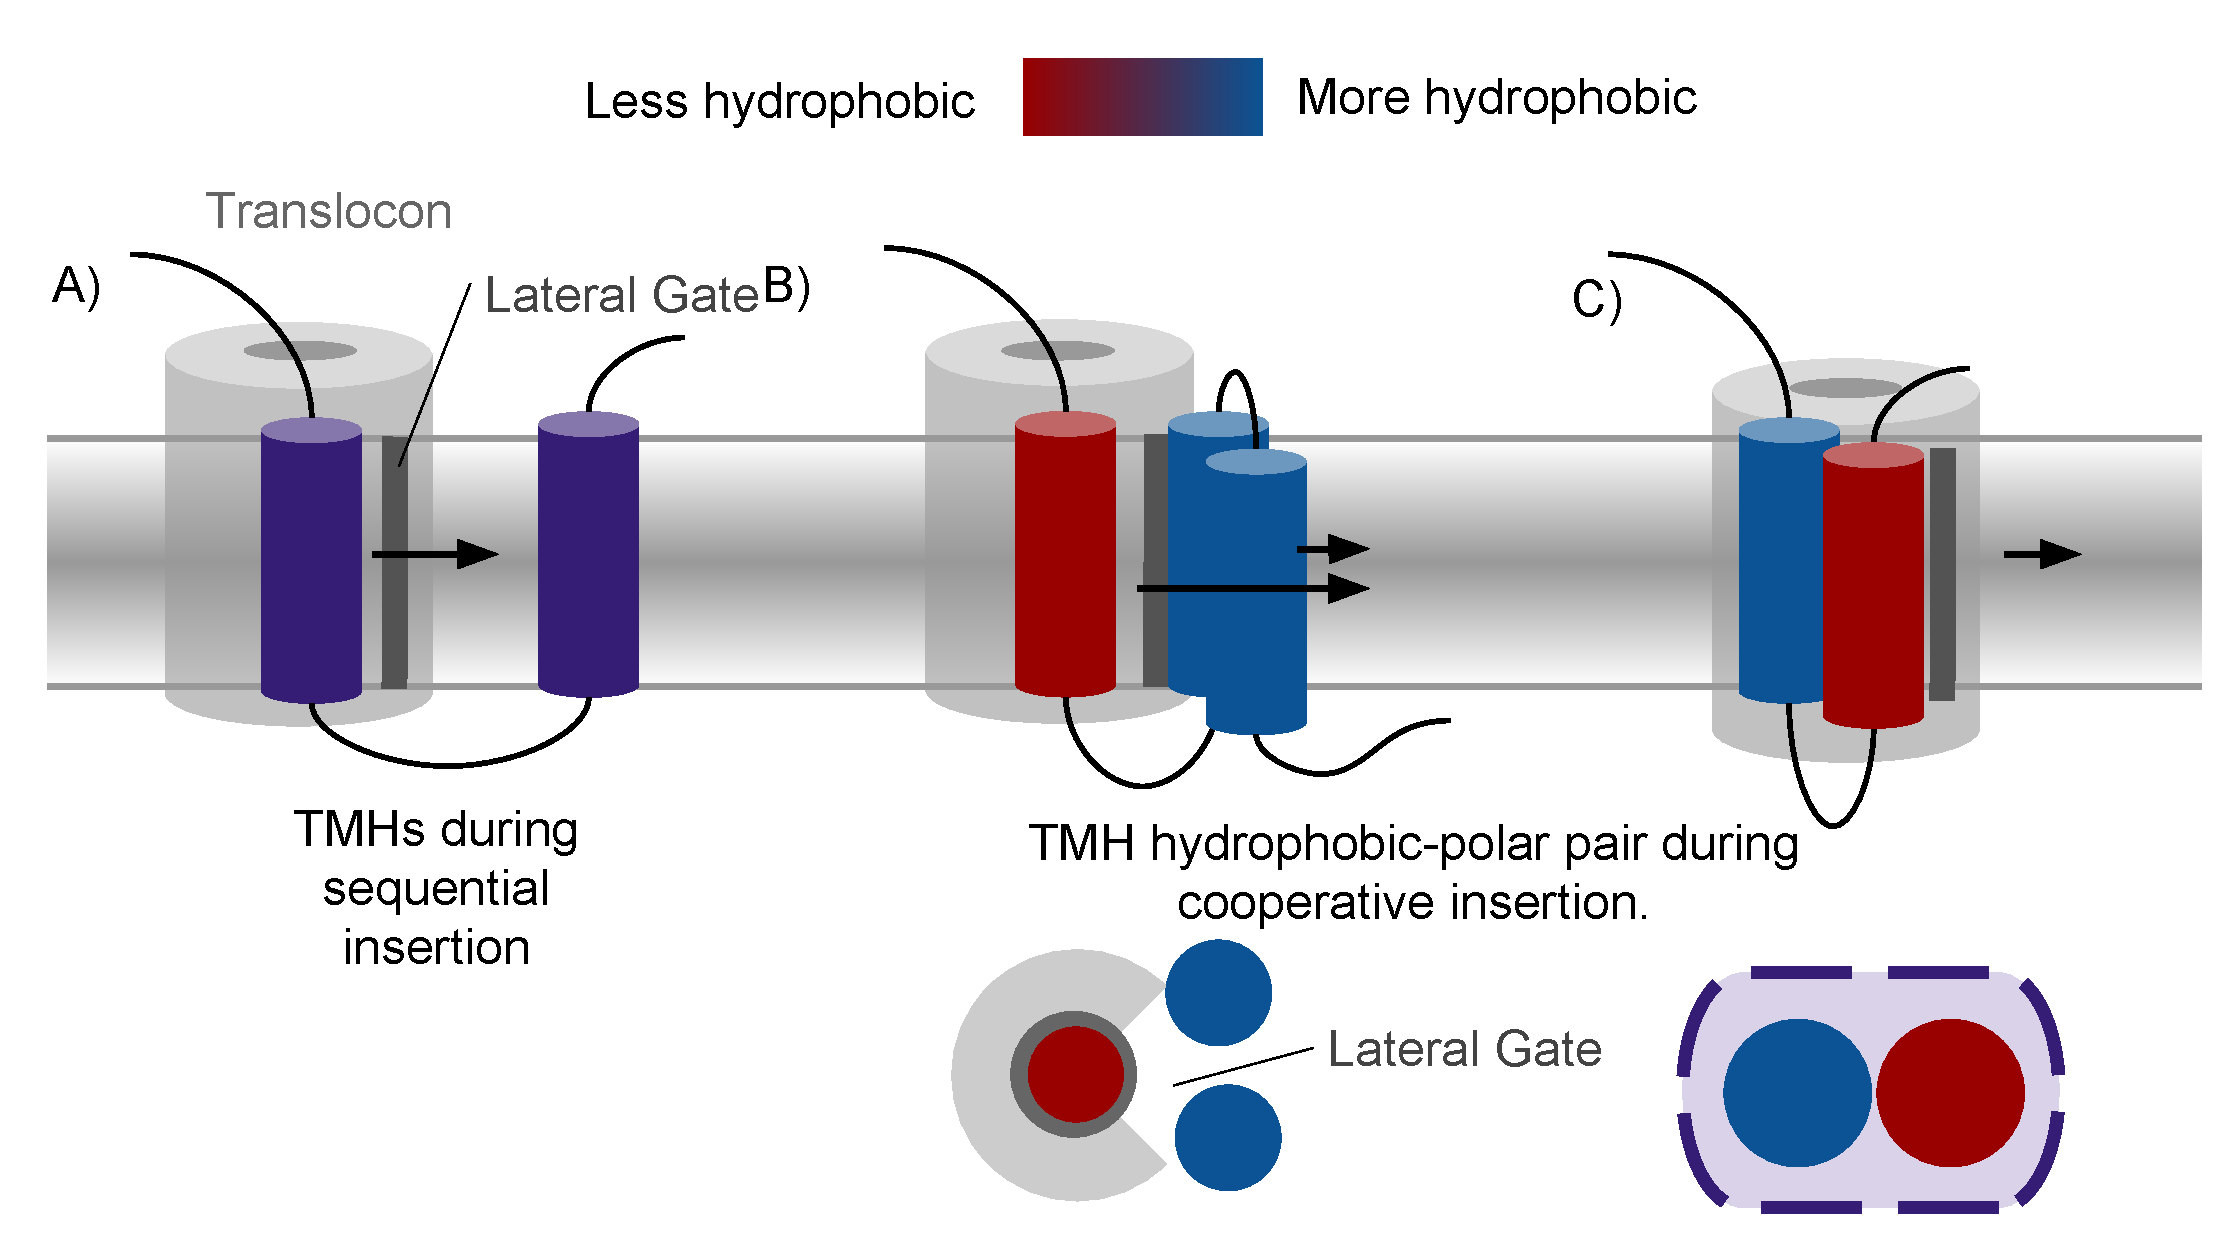
\includegraphics[width=1\textwidth]{multipass-folding/Good-bad-TMH}
		\captionof{figure}[A cartoon of potential cooperative TMH insertion methods.]{\textbf{A cartoon of potential cooperative TMH insertion methods.}}

\label{fig:Good-bad-TMH}
\end{figure}

Seen across a variety of 7TM families with varying functions with datasets built from all membrane types (hence variety).
Suggests a pressure for simpler TMHs to precede more complex ones, repeating every 3-4 TMHs.
The universality points toward translocon behaviour pressure, or thermodynamic stability in the membrane.
Would we expect this behaviour if the translocon acted on only one TMH at a time?

\section{Methods}
\subsection{Datasets}
\subsubsection{Membrane protein families}
This is not an exhaustive search among \gls{tmp}s for all examples of starkly polar \gls{tmh}s conserved among the family.
Instead we show that there is precedent for several, but not all, protein families to contain polar helices and that these polar \gls{tmh}s are sequentially next to typically hydrophobic \gls{tmh}s.
Analysis can only be done if the number of \gls{tmh}s is conserved across the family since different mechanisms are utilised to transmit a signal or transport a molecule across the membrane.

Datasets were attained by querying the UniProt database for controlled vocabulary keywords (Table \ref{table:datasetsizes}) \cite{TheUniProtConsortium2014}.
After filtering our redundant proteins using UniRef50, the datasets were stratified according to the total number of \gls{tmh}s per protein.
Only families with a total N > 20 were included in the analysis, for example, there are ion channels with 12 \gls{tmh}s, but only 16 examples fitted the criteria and were omitted from the study.



\begin{table}[htbp]

  \centering
  \captionof{table}[Dataset sizes of common TMP families of transporters and channels.]{\textbf{Dataset sizes of common TMP families of transporters and channels.}
  The type column refers to the family name.
  The keyword identifier column refers to the specific query term that UniProt uses as the controlled vocabulary identifier.
  UniProt hits refers to the number of SwissProt hits, which are manually curated, however the SwissProt and TrEMBL hits are also given in the brackets.
  The UniRef column denotes how many representative sequences resulted from the UniProt hits, again with the number in the brackets including the TrEMBL hits.
  Because UniRef often returns representatives of splice isoforms as a separate hit, the lists were re-uploaded to UniProtKB to get the final hit.
  The lists are then stratified by the total number of TMHs.
  }

\begin{tabular}{lllllll}
  \footnotesize
Type                     & Keyword Identifier & UniProt Hits   & UniRef Representatives &  UniProtKB & TMHs & Final hits \\
Ion channel              & KW-0407            & 2452 (176417)  & 912 (21024)            & 882                & 4    & 234        \\
                         &                    &                &                        &                    & 6    & 188        \\
                         &                    &                &                        &                    & 24   & 34         \\
Ligand-gated ion channel & KW-1071            & 452 (14051)    & 189 (3055)             & 185                & 6    & 33         \\
Voltage gated channel    & KW-0851            & 683 (27,662)   & 285 (3876)             & 267                & 6    & 97         \\
Calcium channel          & KW-0107            & 272 (5056)     & 128 (1003)             & 120                & 6    & 38         \\
Potassium channel        & KW-0631            & 337 (11852)    & 160 (1893)             & 152                & 6    & 88         \\
Sugar transport          & KW-0762            & 1217 (107721)  & 467 (16748)            & 464                & 12   & 134        \\
Chloride channel         & KW-0869            & 303 (3697)     & 117 (1039)             & 117                & 4    & 50         \\
Ion transport            & KW-0406            & 10264 (443600) & 3070 (42259)           & 3023               & 4    & 338        \\
                         &                    &                &                        &                    & 6    & 390        \\
                         &                    &                &                        &                    & 8    & 162        \\
                         &                    &                &                        &                    & 10   & 189        \\
                         &                    &                &                        &                    & 12   & 292        \\
                         &                    &                &                        &                    & 24   & 35
\end{tabular}
\label{table:datasetsizes}
\end{table}


\subsubsection{GPCR subfamilies}
The 7TMR list is a list distributed by UniProt containing G-receptor linked proteins available at \url{http://www.uniprot.org/docs/7tmrlist.txt} \cite{TheUniProtConsortium2014}.
The entire list contains 3115 UniProt IDs which mapped to 3092 records on the date of download (12/9/2017).
After removing redundant records using UniRef50 to identify cluster representitives, 1142 records made the final dataset.
The original list is also sub categorised by function.
Here, we also looked at opsins, the T2R taste receptors, frizzled/smooth \gls{gpcr}s, metabotropic gluatmate receptors (Family C), fungal mating proteins, and serotonin receptors.

218 opsin records were mapped through UniRef50 to 40 records.
211 T2R taste receptors were mapped to 45 records after UniRef50.
There were 82 records for frizzled/smooth, of which 41 were cluster representitives after querying with UniRef50.
114 were metabotropic glutamate recepters which became 44 after redundancy removal.
In serotonin, 91 original records were represented by 28 records.
There were 13 fungal mating proteins, represented by 9 after UniRef50.



\subsection{Gene Ontology}
77153 protein records matched the query \url{annotation:(type:transmem) AND reviewed:yes} in UniProt \cite{TheUniProtConsortium2014}.
30045 records of these represented those proteins after submitting the list to UniRef50.
To gain an approximate idea of what proteins may have cooperative \gls{tmh}s, we submitted that non-redundant SwissProt transmembrane dataset to PANTHER and used their pie chart visualisation \cite{Mi2017}.
We also submitted a constricted list of the non-redundant SwissProt transmembrane dataset to PANTHER by sorting the list according to proteins with sequentially adjacent \gls{tmh}s that had the greatest difference in Kyte \& Doolittle hydrophobicity \cite{Kyte1982}.
This consisted of the top 102 pairs from a list of 101604 (the top 0.1\%) \gls{tmh} pairs from 87 unique UniProt records.
In PANTHER, these hit 59 genes with 58 functions.

\subsection{Complexity}

\subsection{Statistics}
